\documentclass{rapportCS}
\usepackage{lipsum}
\title{Rapport CentraleSupelec - Template} %Titre du fichier

%%%%%%%%%%%%%%%%%%%%%% LES PACKAGES
%-------------------
% gestion des pages
%-------------------
\usepackage{pdflscape} %pages horizontales dans le PDF
\usepackage{calc} %pour pouvoir écrire \textwidth-1cm


%-------------------
% sommaire 
%-------------------
\usepackage{tocloft}%mise en forme de la toc
\usepackage{titlesec}%mise en forme des titres de section
\usepackage[nottoc, notlof, notlot]{tocbibind}


%-------------------
% langue et encodage
%-------------------
\usepackage[utf8]{inputenc}
\usepackage[T1]{fontenc}
\usepackage[]{babel}
%\usepackage[english]{babel}
%\usepackage[french]{babel}


%-------------------
% symboles et mode maths
%-------------------
\usepackage{amsmath,amsfonts,amssymb}
\usepackage{textcomp,lmodern}%pour l'euro
\usepackage{mathrsfs}%lettres style manuscrit italique


%-------------------
% code
%-------------------
\usepackage{minted}
%%-- pour la commande qui évite l'italique
%%-- voir https://github.com/gpoore/minted/issues/71
%\usepackage{etoolbox}
%\usepackage{newunicodechar}
\usepackage[vlined, french, onelanguage]{algorithm2e}



%-------------------
% environnement, théorèmes et exercices
%-------------------
%\usepackage{thmbox}%pour les jolis thm


%-------------------
% tableaux
%-------------------
\usepackage{array,multirow}


%-------------------
% images
%-------------------
\usepackage{xcolor} %pour redefinir des couleurs
\usepackage{caption}%les personaliser (les centrer par ex)
\usepackage{graphicx} % pour includegraphics

\usepackage{tikz} %graphiques et dessins
\usetikzlibrary{shapes}%pr écrire \node[ellipse] par ex
\usetikzlibrary{positioning} %pr écrire \node[below rigth = 3pt and 5pt]
\usetikzlibrary{decorations.pathreplacing}%pr les accolades
\usetikzlibrary{patterns}%pour les hachures





%-------------------
% divers
%-------------------
\usepackage{cancel}%pour barrer
%-------------------
\usepackage{lipsum}% for dummy text
%-------------------
\usepackage{appendix}%pour les annexes




%%%%%%%%%%%%%%%%%%%%%% MISE EN FORME
%%%%%%%%%%%%%%%%%%%%%%%%%%%%%%%%%%%%%%%%%%%%
% MISE EN FORME DU CODE AVEC MINTED
%%%%%%%%%%%%%%%%%%%%%%%%%%%%%%%%%%%%%%%%%%%%

%pour le style des numéros de ligne minted
\renewcommand{\theFancyVerbLine}{\sffamily
\textcolor{expli}{\scriptsize
\oldstylenums{\arabic{FancyVerbLine}}}}

%pour éviter l'italique 
%car apparaissaient en italique à la fois les commentaires et les includes
\newtoggle{inminted}
\AtBeginEnvironment{minted}{\let\itshape\relax}

%paramètres pour le c
\setminted[c]{
	%--fond et cadre	
	%bgcolor = black!3!white,
	frame = leftline,
	framesep = 6pt,
	rulecolor= expli,
	%--numéro de ligne
	linenos=true,
	numbersep=4pt,
	%stepnumber=2,
	xleftmargin=20pt,%pour que les chiffres débordent pas
	%--découpage des longues lignes
	breaklines=true,
	%--tabulations
	tabsize=2,
	}

%paramètres pour le ocaml
\setminted[ocaml]{
	%--fond et cadre	
	%bgcolor = black!3!white,
	frame = leftline,
	framesep = 6pt,
	rulecolor= expli,
	%--numéro de ligne
	linenos=true,
	numbersep=4pt,
	%stepnumber=2,
	xleftmargin=20pt,%pour que les chiffres débordent pas
	%--découpage des longues lignes
	breaklines=true,
	%--tabulations
	tabsize=2,
	}




%%%%%%%%%%%%%%%%%%%%%%% LA PALETTE DE COULEURS
%%%%%%%%%%%%%% couleurs locales
\definecolor{jaune}{RGB}{255, 195, 0 }
\colorlet{oranger}{orange!50!jaune}
\definecolor{orange}{RGB}{250, 130, 1}

\definecolor{vert}{RGB}{194, 247, 50}
\definecolor{herbe}{RGB}{80, 180, 33}
\definecolor{vertFonce}{RGB}{20, 148, 20} 

\colorlet{vertdEau}{blue!50!green!30!white} 
\definecolor{turquoise}{RGB}{0, 204, 203}
\colorlet{monCyan}{turquoise!90!blue} 
\definecolor{turquoiseFonce}{RGB}{0, 149, 182} 
\colorlet{marine}{blue!60!black}
\colorlet{doubleu}{gray!50!blue}


\colorlet{lavande}{vertdEau!50!blue}
\definecolor{mauve}{RGB}{161, 132, 220}
\definecolor{lilas}{RGB}{154, 107, 165}


\definecolor{prunelle}{RGB}{106,24, 141}
\definecolor{prune}{RGB}{121, 7, 123}
\definecolor{violet}{RGB}{153, 0, 139}
\definecolor{violette}{RGB}{128, 0, 128} 

\definecolor{roseAcidule}{RGB}{255, 0, 127} 
\colorlet{rose}{orange!50!oranger!50!magenta!50!violet}
\definecolor{grenat}{RGB}{141, 24, 59}
\colorlet{framboise}{magenta!90!red!80!black}




\colorlet{ocre}{orange!90!green!80!white} 
\definecolor{chamois}{RGB}{200, 141, 75}

\definecolor{briqueRouge}{RGB}{200, 48, 24}
\definecolor{brique}{RGB}{141, 48, 24}
\definecolor{taupe}{RGB}{165, 137, 107}


\colorlet{expli}{gray}


\colorlet{saumon}{yellow!45!magenta}



%%%%%%%%%%%%%%%%%%%%%%% LES COMMANDES 
%%%%%%%%%%%%%%%%%%%%%%%%%%%%%%%%%%%%%%%%%%%%
% GENERAL  
%%%%%%%%%%%%%%%%%%%%%%%%%%%%%%%%%%%%%%%%%%%%

%raccourcis généraux
\newcommand {\ie}{\textit{i.e}. }
\newcommand {\cf}{\textit{Cf.} }
\newcommand {\resp}{resp.\! }


%pour les belles fonctions (à mettre entre $ $  ou entre $$ $$ )
\newcommand{\fonction}[5]{ 
#1 =
\left( \! \begin{tabular}{c@{ }c@{ }l} 
$#2$  & $\longrightarrow$   & $#3$  \\
$#4$  & $\longmapsto$       & $#5$ 
\end{tabular} \! \right)
}

%le widebar (inutile si package mathabx
\newcommand{\widebar}[1]{\overline{#1}}

%symboles rapprochés
\renewcommand {\=}{\!=\!}
\renewcommand {\-}{\!-\!}
\renewcommand {\:}{\!:\!}
\newcommand {\+}{\!+\!}
\newcommand {\iin}{\!\in\!}
\newcommand {\inclus}{\!\subseteq\!}

%symboles
\newcommand{\bubullet}{-}
\newcommand{\subbullet}{\circ}
\newcommand{\parties}{\mathcal{P}}

%produit scalaire
\renewcommand{\.}{\!\cdot\!}

%indicatrice
\newcommand{\1}{\mathbb{I}}

%cardinal
\newcommand{\card}[1]{\left|#1\right|}

%%%%%%%%%%%%%%%%%%%%%%%%%%%%%%%%%%%%%%%%%%%%
% ENSEMBLES DE NOMBRES & ESPACES DE VARIABLES  
%%%%%%%%%%%%%%%%%%%%%%%%%%%%%%%%%%%%%%%%%%%%

%pour N,Z,R 
\newcommand {\NN}{\mathbb{N}}
\newcommand {\NNe}{\NN^*}
\newcommand {\R}{\mathbb{R}}
\newcommand {\Rp}{\R_+}
\newcommand {\Rpe}{\R^*_+}
\renewcommand {\Re}{\R^*}
\newcommand {\Z}{\mathbb{Z}}


%%%%%%%%%%%%%%%%%%%%%%%%%%%%%%%%%%%%%%%%%%%%
% LES NOUVEAUX OPERATEURS  
%%%%%%%%%%%%%%%%%%%%%%%%%%%%%%%%%%%%%%%%%%%%

%optim
\DeclareMathOperator*{\argmin}{arg\,min}
\DeclareMathOperator*{\argmax}{arg\,max}

%analyse cvx
\DeclareMathOperator*{\conv}{conv}
\DeclareMathOperator*{\extr}{extr}
\DeclareMathOperator*{\vect}{vect}
\DeclareMathOperator*{\aff}{aff}





%%%%%%%%%%%%%%%%%%%%%%%%%%%%%%%%%%%%%%%%%%%%
% ICONES ET SYMBOLES HORS MATHS 
%%%%%%%%%%%%%%%%%%%%%%%%%%%%%%%%%%%%%%%%%%%%
\newcommand{\flch}{\item[$\rightarrow$]}

\newcommand{\attention}{\dbend}

\newcommand{\alamain}{{\LARGE\ding{45}}}

\newcommand{\surmachine}{

\begin{tikzpicture}[scale=0.1]
\draw[line width=1.2pt](-2,0) rectangle (2,3);
\fill(-1,0)--(1,0)--(2,-1)--(-2,-1)--(-1,0);
\end{tikzpicture}
}

\newcommand{\pasapas}{
\begin{tikzpicture}[scale=0.1]
\draw (0,0)--(0,1)--(1,1)--(1,2)--(2,2)--(2,3)--(3,3)--(3,4)--(4,4)--(5,4)--(5,0)--(0,0);
\end{tikzpicture}
}

\newcommand{\afaire}{
\begin{tikzpicture}[scale=0.1]
\draw (0,0)rectangle(4,4);
\end{tikzpicture}
}

\newcommand{\uneetoile}{{\LARGE$*$}\,}
\newcommand{\deuxetoiles}{{\LARGE$*\,*$}\,}
\newcommand{\troisetoiles}{{\LARGE$_*^*$}{\large$*$}\,}


\newcommand{\couleur}[1]{\textcolor{turquoiseFonce!70!black}{#1}}
\newcommand{\important}[1]{\textbf{\couleur{#1}}}

\newtcolorbox{coder}{
enhanced,
boxrule=0pt,frame hidden,
borderline west={4pt}{0pt}{briqueRouge},
colback=black!3!white,
sharp corners
}
\newtcolorbox{codeb}{
enhanced,
boxrule=0pt,frame hidden,
borderline west={4pt}{0pt}{vertdEau},
colback=black!3!white,
sharp corners
}

\newcommand{\intervalle}[2]{[\![#1,#2]\!]}

\renewcommand{\appendixpagename}{Annexes}
\renewcommand{\appendixtocname}{Annexes}
%%%%%%%%%%%%%%%%%%%%%%%
\newcounter{chapter}
\newcounter{thm}

\usepackage{mathtools, amssymb}
\usepackage[thmmarks, amsmath]{ntheorem}
\usepackage{cleveref}

%------------------------------------------------
% Théorèmes et leurs variantes
\theoremstyle{plain}
\theoremheaderfont{\upshape\bfseries}
\theorembodyfont{\itshape}
\theoremseparator{\textbf{.\,---}}
\newtheorem{theoreme}{Théorème}[chapter]
\newtheorem{corollaire}[thm]{Corollaire}
\newtheorem{lemme}[thm]{Lemme}

%------------------------------------------------
% Définitions et environnements similaires
\theoremheaderfont{\bfseries}
\theorembodyfont{\mdseries\upshape}
\theoremseparator{.}
\theoremstyle{definition}
\newtheorem{definition}{Définition}[chapter]
\newtheorem{exemple}{Exemple}[chapter]
\newtheorem{exo}{Exercice}[chapter]
\newtheorem{propriete}{Propriété}[chapter]

%------------------------------------------------
% Démonstrations
\theoremstyle{nonumberplain}
\theoremheaderfont{\mdseries\upshape}
\theoremsymbol{$\mathrm{o}.\varepsilon.\delta.$}
\theoremheaderfont{\scshape}
\theoremseparator{\,:}
\newtheorem{dem}{Démonstration}

% Ajustement de cleveref pour chaque type de théorème
\crefname{theoreme}{Théorème}{Théorèmes}
\crefname{corollaire}{Corollaire}{Corollaires}
\crefname{lemme}{Lemme}{Lemmes}
\crefname{definition}{Définition}{Définitions}
\crefname{exemple}{Exemple}{Exemples}
\crefname{exo}{Exercice}{Exercices}
\crefname{propriete}{Propriété}{Propriétés}
\crefname{dem}{Démonstration}{Démonstrations}

% Ajustement des formats de référence pour cleveref
\crefformat{theoreme}{#2Théorème~#1#3}
\crefformat{corollaire}{#2Corollaire~#1#3}
\crefformat{lemme}{#2Lemme~#1#3}
\crefformat{definition}{#2Définition~#1#3}
\crefformat{exemple}{#2Exemple~#1#3}
\crefformat{exo}{#2Exercice~#1#3}
\crefformat{propriete}{#2Propriété~#1#3}
\crefformat{dem}{#2Démonstration~#1#3}

\setcounter{chapter}{1}
\setcounter{thm}{1}






%%%%%%%%%%%%%%%%%%%%%%%%%%%%%%%%%%%%%%%

\begin{document}

%----------- Informations du rapport ---------

\logoentreprise{logos/logoGraphene.png}

\titre{Morphing} % Titre du fichier

\mention{Cursus ingénieur} % Nom de la Mention
\trigrammemention{ING1} % Pour le bas de la page
\master{Génie informatique} % Nom du master
\filiere{Première année} % Nom de la filière

\eleve{Ryan Bouchou, X\\X, X\\X}

\dates{20 janvier 2024}

% Informations tuteurs écoles
%%\tuteurecole{
%    Mention : \textsc{Prénom Nom} \\
%    prenom.nom@centralesupelec.fr \\
%    Filière : \textsc{Prénom Nom} \\ 
%    prénom.nom@gmail.com 
%} 

\tuteurentreprise{
    \textsc{Élisabeth X} \\
    prénom.nom@entreprise.com 
}


%----------- Initialisation -------------------
        
\fairemarges %Afficher les marges
\fairepagedegarde %Créer la page de garde

%----------- Résumé -------------------
\vspace*{\stretch{1}}
\begin{center}
	\begin{abstract}
        
    \end{abstract}
\end{center}
\vspace*{\stretch{1}}
\newpage

%------------ Table des matières ----------------
\newpage
\bgroup
\pagestyle{empty}
\makenomenclature
\pagestyle{fancy}
\fancyheadoffset{0.5cm}
\lhead{
\includegraphics[scale=0.2]{logos/CSxParisSaclay.jpg}} %Affichage de l'image au top de la page
\rhead{\nouppercase{\leftmark}}
\cfoot{\textbf{\titre}}
\rfoot{}
\lfoot{\trigrammemention}
\tabledematieres 
\clearpage
\egroup 


%%%%%%%%%%%%%%%%%%%%%%%%%%%%%
%    Corps du rapport       %
%%%%%%%%%%%%%%%%%%%%%%%%%%%%%

\section{Cas des polygones simples}
\label{sec:polygones-simples}
En premier lieu, nous allons nous intéresser au cas des polygones simples.
Ce faisant, ceci sera l'occasion pour nous de faire notre premier pas dans l'\emph{informatique graphique},
en traitant des cas élémentaires du problème de la morphose.
\subsection{Généralités} 
\label{sec:generalites}
\paragraph{Conventions}
Pour toute la suite, et sauf mention contraire, on se place dans le $\R$-evn $\R^2$ muni de la norme euclidienne.
On notera pour tout vecteur $x\in\R^2$, $X\in \mathcal{M}_{2,1}(\R)$ la matrice colonne associée à $x$ dans la base canonique de $\R^2$.

\begin{definition}\label[definition]{def:1}
    Soit $n$ un entier naturel non nul. On appelle \emph{polygone simple} de $\R^2$ tout $n$\_uplet $P=(p_1,\ldots,p_n)$ de $\R^2$ tels que:
    \begin{enumerate}
        \item Les segments ne se croisent pas, c'est-à-dire que pour chaque paire de segments \( [p_i, p_{i+1}] \) et \( [p_j, p_{j+1}] \) (où \( p_{n+i} \) est \( p_i \)), les segments ne partagent pas de points autres que les sommets.
        \item Chaque sommet $p_i$ est partagé par exactement deux segments.
    \end{enumerate}
    On notera $p_{i^+}$ le segment $[p_i, p_{i+1}]$ et $p_{i^-}$ le segment $[p_i, p_{i-1}]$. Enfin, on notera $\mathbb{P}$ l'ensemble des polygones simples de $\R^2$.
\end{definition}

\begin{definition}\label[definition]{def:2}
    Soit $P\in\mathbb{P}$ un polygone simple de $\R^2$.
    \begin{enumerate}
        \item On appelle \emph{ordre} de $P$ le nombre $n$ de composantes de $P$.
        \item On appelle \emph{arête} de $P$ tout segment $p_{i^+}$ ou $p_{i^-}$ pour $i\in\{1,\ldots,n\}$. 
        \item On appelle \emph{sommet} de $P$ tout vecteur $p_i$ pour $i\in\{1,\ldots,n\}$.
    \end{enumerate}
    Subséquemment, pour $n$ un entier naturel non nul, on note $\mathbb{P}_n$ l'ensemble des polygones simples de $\R^2$ d'ordre $n$.

\end{definition}

\begin{definition}\label[definition]{def:3}
    Soit $P\in\mathbb{P}$ un polygone simple de $\R^2$.
    On appelle \emph{intérieur} de $P$, noté $\overset{\circ}{P}$ , l'ensemble des points $x\in\R^2$ tels que $x$ est à gauche de chaque arête de $P$.
\end{definition}




\paragraph{Situation} À ce stade, l'enjeu de cette première partie est de déterminer un algorithme permettant 
la morphose d'un polygone simple $P$ vers un autre polygone simple $Q$. Pour ce faire, il nous faut nous intéresser
aux conditions d'une telle transformations, ainsi qu'à sa réalisation.

\subsection[Morphing naif]{Un premier algorithme de morphing}
\label{sec:morphing-naif}
\subsubsection{Principe et notation}
\paragraph{Principe} L'idée de cet algorithme est de déformer progressivement le polygone $P$ en un autre polygone $Q$.
Pour ce faire, une première approche consiste à déformer chaque sommet $p_i$ de $P$ en un sommet $q_i$ de $Q$ par
une interpolation linéaire. Ainsi, on obtient une suite de polygones $(P_{k})_{0\leq k\leq N}$ 
où $N$ est le nombre d'images intermédiaires voulues et tels que $P_{0}=P$, $P_{N}=Q$.

\begin{coder}
    Pour que l'algorithme soit correct, il est nécessaire que les polygones $P$ et $Q$ soient de même ordre.
\end{coder}

\paragraph*{Notation} Soit $n,N>0$ et $(P_k)_{0\leq k\leq N}$ une suite de polygones de $(\mathbb{P}_{n})^{\NN}$.
 On notera $p^{(k)}_1,\ldots,p^{(k)}_n$ les sommets de $P_k$.

\paragraph{} Ce faisant, pour le calcul des images intermédiaires on donne l'algorithme suivant:\\[0.5cm]
\begin{algorithm}[H]
    \caption{générationFramesNaif}\label{alg:0}
    \SetAlgoLined
    \KwData{$P,Q\in\mathbb{P}_n$ deux polygones, $N>0$ le nombre de frames}
    \KwResult{Une suite de polygones $(P_k)$}
    $P^*\gets(P_1,\dots,P_N)$\\
    \For{$k\gets 0$ \KwTo $N$}{
        $t\gets\frac{k}{N}$\\
        $P_k=(p^{(k)}_1,\ldots,p^{(k)}_n)$\\ 
        \For{$i\gets 1$ \KwTo $n$}{
            $p^{(k)}_{i}\gets (1-t)*p_i+t*q_i$
        }
    }
    \Return $P^*$
\end{algorithm}

\subsubsection{Cas des images matricielles}
\paragraph{Principe} Dans le cadre de l'exercice, la donnée du problème est consituée de deux images matricielles $P$ et $Q$
de taille $L\times l$ représentant respectivement des polygones simples de couleur même couleur. Naturellement,
plusieurs méthodes algorithmiques peuvent être utilisées pour encoder l'information géométrique portée par une image.
Entre autre, des algorithme de \emph{détection de contours} ou de \emph{segmentation} peuvent être utilisés. Toutefois, et par soucis
de simplicité, nous allons considérer que l'information géométrique est directement encodée par l'utilisateur lors de la saisie des
\emph{points de contrôle}. De plus, pour chaque pixel de coordonnées $(i,j)$, on a :

$$
\begin{cases}
    \1_{P}(i,j) \= 1 & \text{si } (i,j)\in\overset{\circ}{P}\\
    \1_{P}(i,j) \= 0 & \text{sinon}
\end{cases}
$$
\begin{coder}
    Pour que l'algorithme soit correct, il est nécessaire que les images $P$ et $Q$ soient de même taille. De plus,
    si les points de contrôle saisis par l'utilisateur ne correspondent pas aux sommets des polygones,
    les résultats de l'algorithme peuvent être inattendus.
\end{coder}

\begin{propriete}\label[proprieté]{prop:1}
    Soit $u,v\in\R^2$ deux vecteurs.
    Alors $u$ est à gauche de $v$ si et seulement si $det(u,v)>0$.
\end{propriete}
\begin{dem}
    Admis.
\end{dem}


\begin{propriete}\label[proprieté]{prop:1}
    Soit $p=[u,v], (u,v)\in\R^2$ un segment et $x\in\mathbb{R}^2$ un vecteur.
    Alors $x$ est à gauche de $p$ si et seulement si $det(p,[u,x])>0$.
\end{propriete}
\begin{dem}\label{dem:1}
    Soit $u,v\in\R^2$ deux vecteurs. On note $\theta$ l'angle orienté entre $u$ et $v$.
    Alors, 
    \begin{align}
        u \text{ est à gauche de } v &\iff \text{det}(u,v)>0\\
        &\iff \left\lVert u \right\rVert \cdot \left\lVert v \right\rVert \sin(\theta)>0\\
        &\iff \sin(\theta)>0\\
        &\iff \theta\in\left]0,\pi\right[\\
        &\iff u \text{ est dans le demi-espace à gauche de } v
    \end{align}
\end{dem}
\paragraph{} Ce faisant, pour le calcul des images intermédiaires, 
et la determination de l'intérieur du polygone, de on donne la suivante:\\[0.5cm]
%% Détermination de l'intérieur d'un polygone

\begin{algorithm}[H]
    \SetAlgoLined
    \KwData{Une liste de points $tab$ représentant le polygone, un point $P$}
    \KwResult{Un booléen indiquant si le point $P$ est à l'intérieur du polygone}
    
    $nbp \gets \text{taille de } tab$ 
    \For{$i \gets 0$ \KwTo $nbp-1$}{
        $A \gets tab[i]$ 
        $B \gets tab[(i+1) \mod nbp]$ 
        
        $D \gets (B.x - A.x, B.y - A.y)$ 
        $T \gets (P.x - A.x, P.y - A.y)$ 
        
        $d \gets det(D,T)$ 
        
        \If{$d < 0$}{
            \Return Faux 
        }
    }
    \Return Vrai;
    
    \caption{isInside}
\end{algorithm}

\paragraph{} On en déduit l'algorithme naif pour le mophing de formes unies simples:\\[0.5cm]

\begin{algorithm}[H]
    \SetAlgoLined
    \KwData{Deux images matricielles $P$ et $Q$ de taille $L\times l$, un entier $N$}
    \KwResult{Une suite d'images matricielles $P^*$}
    
    $nbp \gets \text{taille de } tab$\\
    $P^* \gets \text{générationFramesNaif}(P,Q)$\\
    \For{$i \gets 0$ \KwTo $nbp-1$}{
        \For{$x \gets 0$ \KwTo $L-1$}{
            \For{$y \gets 0$ \KwTo $l-1$}{
                if($isInside(P^*_i, (x,y))$){
                    $P^*_i[x][y] \gets color$
                }
            }
        }

    }
    \Return $P^*$
    
    \caption{morphingNaif}
\end{algorithm}
\newpage
\paragraph{Résultats} Considérons une exécution de l'algorithmes sur deux instances du problème.\\
\begin{figure}[h!]
        \centering
        \begin{subfigure}{0.4\textwidth}
            \centering
            
\includegraphics[width=0.8\textwidth]{img/p1/1.png}
            \caption{Image initiale}
        \end{subfigure}
        \begin{subfigure}{0.4\textwidth}
            \centering
            
\includegraphics[width=0.8\textwidth]{img/p1/2.png}
            \caption{Image intermédiaire 1}
        \end{subfigure}
        \begin{subfigure}{0.4\textwidth}
            \centering
            
\includegraphics[width=0.8\textwidth]{img/p1/3.png}
            \caption{Image intermédiaire 2}
        \end{subfigure}
        \begin{subfigure}{0.4\textwidth}
            \centering
            
\includegraphics[width=0.8\textwidth]{img/p1/4.png}
            \caption{Image intermédiaire 3}
        \end{subfigure}
        \begin{subfigure}{0.4\textwidth}
            \centering
            
\includegraphics[width=0.8\textwidth]{img/p1/5.png}
            \caption{Image intermédiaire 4}
        \end{subfigure}
        \begin{subfigure}{0.4\textwidth}
            \centering
            
\includegraphics[width=0.8\textwidth]{img/p1/6.png}
            \caption{Image finale}
        \end{subfigure}
        \caption{Résultats de l'algorithme de morphing}
\end{figure}

\begin{codeb}
    Dans le cas de polygones simples, relativements semblables dans leur géométrie, 
    l'algorithme de morphing naif donne des résultats satisfaisants.
\end{codeb}

\paragraph{En pratique} Toutefois, il apparaît qu'une telle approche ne préserve pas les propriétés géométriques
du polygone. En effet, les images intermédiaires peuvent contenir des segments qui se croisent, 
ou des sommets qui ne sont pas partagés par exactement deux segments. Dans un tel cas, la transformations
ne paraît pas naturelle.
\begin{figure}[h!]
    \centering
    
\includegraphics{img/p1/naif.png}
    \caption{Interpolation linéaire, observez les auto-intersections. \cite{cornillac2010morphing}}
\end{figure}
\newline
Ainsi, il est nécessaire de trouver une approche plus rigoureuse pour le morphing de polygones simples.

\subsection[Méthode L-A]{Morphing par interpolation longeur-angle}

\subsubsection{Principe et notation}
\paragraph{Principe} L'idée de cette méthode, issue des travaux de Sederberg \cite{sederberg1993}, est de déformer progressivement le polygone $P$ en un autre polygone $Q$, en interpolant
linéairement la mesure des angles entre chaque arêtes consécutives, et leurs normes respectives. Ce faisant, l'avantage est de préserver les propriétés géométriques
 souhaitées pour un rendu visuel naturel. On parle d'\emph{invariance par mouvement rigide}.
 de morphing améliorée est.

\paragraph*{Notation} Soit $n,N>0$ et $(P_k)_{0\leq k\leq N}$ une suite de polygones de $(\mathbb{P}_{n})^{\NN}$.
On pose, pour $k\in\{0,\ldots,N\}$:
\begin{itemize}
    \flch $l^{(k)}_i$ la longueur de l'arête $p^{(k)}_{i^{+}}$,
    \flch $\theta^{(k)}_i$ l'angle entre les arêtes $p^{(k)}_{i^{-}}$ et $p^{(k)}_{i^{+}}$.
\end{itemize}
Subséquemment, pour une image intermédiaire $k \in \{0,\ldots,N\}$, avec $t=\frac{k}{N}$ on a:

\begin{align*}
        l^{(k)}_i &= (1-t)l_i+tq_i\\
        \theta^{(k)}_i &= (1-t)\theta_i+t\theta_i
\end{align*}

\paragraph{} Ce faisant, pour le calcul des images intermédiaires on donne l'algorithme suivant:

\begin{algorithm}[H]
    \caption{générationFramesLA}\label{alg:1}
    \SetAlgoLined
    \KwData{$P,Q\in\mathbb{P}_n$ deux polygones, $N>0$ le nombre de frames}
    \KwResult{Une suite de polygones $(P_k)$}
    $P^*\gets(P_1,\dots,P_N)$\\
    $P_0\gets P$, $P_N\gets Q$\\
    \For{$k\gets 0$ \KwTo $N$}{
        $t\gets\frac{k}{N}$\\
        $P_k=((l^{(k)}_1,\theta^{(k)}_1),\ldots,(l^{(k)}_n,\theta^{(k)}_n))$\\ 
        \For{$i\gets 1$ \KwTo $n$}{
            $l^{(k)}_i\gets (1-t)l_i+tq_i$\\
            $\theta^{(k)}_i\gets (1-t)\theta_i+t\theta_i$
        }
    }
    \Return $P^*$
\end{algorithm}

\subsubsection{Cas des images matricielles}
\begin{codeb}
    En l'état, et de par des contraintes de temps, nous n'avons pas implémenté ce segond algorithme. On donne cependant une comparaison des résultats obtenus par \emph{Sederberg et al} \cite{sederberg1993} avec les deux méthodes.
\end{codeb}

\begin{figure}[h!]
    \centering
    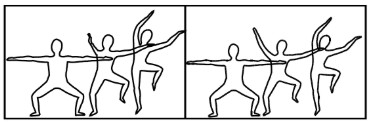
\includegraphics{img/p1/la.png}
    \caption{Morphing par interpolation longueur-angle à droite, naive à gauche. \cite{sederberg1993}}
\end{figure}

%%%%%%%%%%%%%%%%%%%%%%%%%%%%%
%       Liste des Algos     %
%%%%%%%%%%%%%%%%%%%%%%%%%%%%%
\newpage
\listofalgorithms

%%%%%%%%%%%%%%%%%%%%%%%%%%%%%
%       Liste des figures   %
%%%%%%%%%%%%%%%%%%%%%%%%%%%%%
\newpage
\listoffigures

%%%%%%%%%%%%%%%%%%%%%%%%%%%%%
%           Annexe          %
%%%%%%%%%%%%%%%%%%%%%%%%%%%%%
\newpage
\appendix  % Début des annexes
\appendixpage  % Page de titre pour les annexes
\addappheadtotoc  % Ajouter la page des annexes à la table des matières
\section[Splines]{Morphing de courbes splines}
\begin{algorithm}
    \tcp{Trouve l'intervalle dans le vecteur de noeuds qui contient le paramètre u}
    \SetKwFunction{FMain}{trouverIntervalle}
    \SetKwProg{Fn}{Fonction}{:}{}
    \Fn{\FMain{$u$, $nodeVector$}}{
        $n \leftarrow nodeVector.size() - 1$\;
        \If{$u \geq nodeVector.get(n)$}{
            \Return{$n - 1$}\;
        }
        \For{$i \leftarrow 0$ \KwTo $n - 1$}{
            \If{$u \geq nodeVector.get(i)$ \textbf{and} $u < nodeVector.get(i + 1)$}{
                \Return{$i$}\;
            }
        }
        \Return{$-1$} \tcp{Interval not found}
    }
    \caption{Trouver intervalle}
    \label{algo:trouver-intervalle}
\end{algorithm}  % Inclusion du fichier d'annexes

%%%%%%%%%%%%%%%%%%%%%%%%%%%%%
%       Bibliographie       %
%%%%%%%%%%%%%%%%%%%%%%%%%%%%%
\newpage
\bibliographystyle{plain}
\bibliography{biblio.bib}
\end{document}
